\documentclass[10pt,conference]{IEEEtran}
\usepackage[utf8]{inputenc}
\usepackage[T1]{fontenc}
\usepackage{cite}
\usepackage{url}
\usepackage{booktabs}
\usepackage{tabularx}
\usepackage{balance}
\usepackage{array}
\usepackage{graphicx}
\usepackage{tikz}

\usetikzlibrary{arrows.meta,positioning,calc}
\def\tightlist{}
\title{Towards Rapid Prototyping of Software Architecture Assistants}

\author{\IEEEauthorblockN{Anonymous Author(s)}
}


\begin{document}
\maketitle
\begin{abstract}
LLM-based software architecture assistants combine domain knowledge, methodological guidance, artifacts, and runtime-specific orchestration. Engineers commonly build them either as bespoke applications on agent frameworks or by manually specializing general-purpose agent harnesses. Both strategies can tie a workflow to an execution environment and make later changes costly. This paper presents HarnessWeaver, a model-based approach for specifying and prototyping domain-specific agentic workflows as LLM-based assistants. Its intermediate HarnessSpec makes intent, domain concepts, methodology, artifacts, and runtime requirements explicit; target materializers use that specification to produce runtime-specific workflows.

We examine two architecture workflows, ATAM evaluation and SARA architecture design, materialized for Claude Code and DeepAgents. For ATAM, both HarnessWeaver targets produced draft reports that passed configured external checks after manual corrections. For SARA, both HarnessWeaver targets completed four stages and selected A3, though their rationales differed. Two executions of the Revfactory Claude baseline selected different alternatives (A3 and A1), despite using the same generated bundle and case. SARA had no domain-specific checker or evaluator-only references. The results provide preliminary evidence for multi-runtime workflow prototyping and expose limits in validation, runtime parity, and execution repeatability.
\end{abstract}
\begin{IEEEkeywords}
agentic workflows; software architecture techniques; model-based AI engineering, design assistants.
\end{IEEEkeywords}
\section{Introduction}

Agentic software is increasingly used for work that extends beyond code generation, including research, analysis, and design. Engineering a useful domain-specific assistant requires more than a capable model: the system must encode a method, provide domain knowledge, manage intermediate artifacts and state, coordinate model calls, and enforce review or completion conditions. In software architecture, for example, an assistant may need to elicit drivers, analyze alternatives against scenarios, preserve evidence provenance, and leave decisions to an architect.

Two construction strategies are common. A team can implement a bespoke agentic application on a framework such as LangChain or LangGraph, directly encoding state, control flow, tools, and artifact handling. Alternatively, it can specialize a general-purpose harness by assembling skills, subagents, and orchestration patterns. The first offers implementation control but ties the method to application code. The second may reuse native harness capabilities, but still requires engineers to translate domain and methodological requirements into runtime-specific structures. In both cases, a team can commit early to a runtime and incur rework when the method or target environment changes.

This paper explores an intermediate engineering layer: \textbf{HarnessWeaver}. Authors describe the intended work, domain, methodology, artifacts, and constraints in runtime-independent sources. A coding agent uses these sources and generation skills to elaborate a HarnessSpec, then materializes one or more target-specific agentic workflows (LLM-based assistants). The specification makes the transition between authored intent and runtime realization inspectable and supports iterative design. The current approach does not search a design space for an optimal workflow, automatically learn a generator, or select a best runtime.

This paper offers three elements for discussion:

\begin{enumerate}
\def\labelenumi{\arabic{enumi}.}

\item
  We describe a model-based approach for specifying domain-specific agentic workflows, keeping methodology state distinct from runtime execution state.
\item
  We outline target-specific materializations for Claude Code and DeepAgents, including orchestration and artifact contracts.
\item
  We report qualitative ATAM and SARA cases and discuss the validation and runtime-parity questions raised by their executions.
\end{enumerate}

The paper is positioned as a new-idea and preliminary feasibility contribution. The CAIN 2027 short research category accommodates research-oriented position or new-idea papers that are not yet fully evaluated, with preliminary results appropriate to the format.

\section{Background and Related Approaches}

\subsection{Methods encoded in multi-agent workflows}

Multi-agent systems often encode a process through roles, prompts, and ordered or delegated tasks. MetaGPT, for example, uses software-development Standardized Operating Procedures (SOPs) to coordinate role-based agents and validate intermediate work \cite{metagpt}. This line of work demonstrates the value of making a workflow explicit within an agent system. HarnessWeaver shares the premise that method and intermediate artifacts matter, while focusing on an engineering representation that can be mapped to different harness technologies. Its methodology model describes activities, readiness, artifacts, semantic state, validation, and completion independently of a particular agent role or orchestration API.

\subsection{Specializing general-purpose harnesses}

General-purpose coding and agent harnesses can be specialized through project instructions, skills, subagents, tools, and orchestration. The Revfactory \texttt{harness} project provides a close practical antecedent: its meta-skill designs domain-specific teams and skills, supports several execution patterns, and includes an evolution workflow \cite{revfactory}. Its companion study reports an author-run controlled experiment on 15 software-engineering tasks and argues that structured preconfiguration can improve agent output \cite{hwang}. This supports the motivation for explicit harness configuration, but also leaves harness construction and adaptation as engineering work. HarnessWeaver builds on this lineage; its generation skills are derived from Revfactory/harness and should not be presented as wholly independent invention. Its focus is the shared intermediate specification and explicit mapping across runtime targets.

The Claude Code skills mechanism and the DeepAgents framework represent different ways to package specialized guidance and execution. DeepAgents supplies general-purpose capabilities such as planning, filesystem access, and subagent delegation \cite{deepagents}. HarnessWeaver uses these native capabilities as target mechanisms rather than attempting to replace them. The contribution under investigation is how domain and methodology descriptions can guide target-specific materialization while preserving a common source model.

\subsection{Domain-specific agentic workflows and harnesses}

AutoOPT is a domain-specific workflow for optimization research. It combines numerical method design through BnB-PEP, LLM-based discovery of analytical descriptions and proofs, Lean 4 verification, and human interpretation; its authors report two case studies with machine-checked theorems \cite{autoopt}. AutoOPT shows how expert methodology can structure an LLM-based research assistant. HarnessWeaver addresses an adjacent engineering question: how to represent a domain workflow and materialize it for different runtime environments.

EvoSafeHarness is closer to harness synthesis. Given a frozen model and domain specification, it jointly evolves a natural-language safety policy and executable enforcement logic using behavioral feedback and adversarial review, and evaluates the resulting safety--utility trade-off \cite{evosafe}. Its objective is deployment-specific safety optimization. The present HarnessWeaver prototype instead describes and maps agentic workflows; it does not optimize policies or generate executable enforcement code. Together, these systems illustrate distinct meanings of ``domain-specific harness'' and motivate further work on the boundary between a workflow specification, its assistant realization, and the surrounding harness.

\subsection{Software architecture assistants}

Prior work has explored LLM-based support for software architecture design and architecture exploration. D\'iaz-Pace et al. introduced ReArch for architecture exploration and reflection with LLM-based agents, using textual system and requirement descriptions as inputs \cite{rearch}. Cervantes et al. describe a broader, ADD-guided design process in which an LLM and architect persona produce an iteration plan and architecture document; they evaluate its outputs against a proven solution and through review by four professional architects \cite{bettertogether}. These works illustrate agentic architecture exploration and end-to-end design workflows. HarnessWeaver addresses a complementary engineering concern: representing such domain methods independently of a runtime and materializing them as assistant workflows. We include SARA, a follow-up architecture-design workflow associated with the ReArch case-study line, as a second domain alongside ATAM evaluation.

\begin{table*}[t]
\centering\footnotesize\renewcommand{\arraystretch}{1.15}
\begin{tabularx}{\textwidth}{>{\raggedright\arraybackslash}X >{\raggedright\arraybackslash}X >{\raggedright\arraybackslash}X >{\raggedright\arraybackslash}X}
\toprule
Approach & Primary engineering unit & Runtime relationship & Relevance to this work\tabularnewline
\midrule
Bespoke agent application & Application code, state, and control flow & Usually chosen at implementation time & Direct control; often couples method to a host\tabularnewline
Manual harness specialization & Skills, agents, tools, and orchestration & Native to a selected general harness & Reuses runtime capabilities; requires manual translation\tabularnewline
MetaGPT / SOP-based systems & Roles and workflow procedures & Framework-specific realization & Makes process and intermediate work explicit\tabularnewline
Revfactory/harness & Generation and evolution skill for Claude Code teams & Primarily Claude Code targets & Closest practical antecedent; source of design lineage\tabularnewline
Better Together & ADD-guided architecture design process and artifacts & LLM with architect persona and human architects & Substantive architecture-design workflow; not a cross-runtime materializer\tabularnewline
AutoOPT & Staged optimization-research workflow with numerical and formal tools & LLMs, BnB-PEP, Lean 4, and human review & Domain-specific research assistant; not a cross-runtime materializer\tabularnewline
EvoSafeHarness & Model/domain-specific policy and code synthesis & Feedback-guided safety optimization & Close harness-synthesis work, with a safety objective\tabularnewline
HarnessWeaver (proposed) & Runtime-independent HarnessSpec & Multiple target adapters & Separates authored method/domain model from realization\tabularnewline
\bottomrule
\end{tabularx}
\end{table*}

\textbf{Table I.} Comparison of construction approaches at the level relevant to this paper. The categories are intentionally broad; they do not imply that each prior system lacks internal abstractions.

\section{HarnessWeaver Approach}

HarnessWeaver treats agentic-workflow construction as a model-to-realization process. Authors provide runtime-independent source material; a generation skill guides an interactive design process; the resulting HarnessSpec describes the intended workflow; target-specific materializers turn it into runtime-native assistant instructions and configuration; and bundle and execution checks provide feedback for revision.

\begin{figure}[t]
\centering
\resizebox{\columnwidth}{!}{%
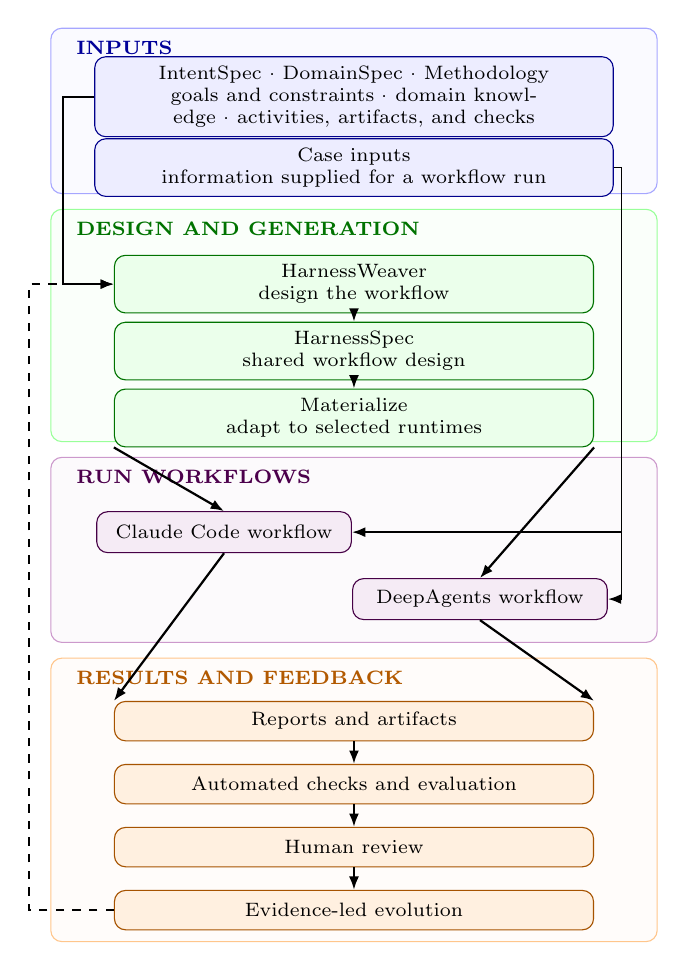
\begin{tikzpicture}[
  x=1cm,y=1cm,
  input/.style={draw,rounded corners,align=center,text width=6.35cm,minimum height=0.54cm,font=\scriptsize,fill=blue!7,draw=blue!55!black},
  design/.style={draw,rounded corners,align=center,text width=5.85cm,minimum height=0.52cm,font=\scriptsize,fill=green!8,draw=green!45!black},
  runtime/.style={draw,rounded corners,align=center,text width=5.2cm,minimum height=0.52cm,font=\scriptsize,fill=violet!8,draw=violet!55!black},
  result/.style={draw,rounded corners,align=center,text width=5.85cm,minimum height=0.5cm,font=\scriptsize,fill=orange!12,draw=orange!65!black},
  arrow/.style={-{Latex[length=1.7mm]},thick},
  feedback/.style={-{Latex[length=1.7mm]},thick,dashed}
]
% Single-column, top-to-bottom rendering of the architecture.md flow.
\fill[blue!2,rounded corners] (0,9.15) rectangle (7.7,11.25);
\draw[blue!35,rounded corners] (0,9.15) rectangle (7.7,11.25);
\fill[green!2,rounded corners] (0,6.0) rectangle (7.7,8.95);
\draw[green!40,rounded corners] (0,6.0) rectangle (7.7,8.95);
\fill[violet!2,rounded corners] (0,3.45) rectangle (7.7,5.8);
\draw[violet!40,rounded corners] (0,3.45) rectangle (7.7,5.8);
\fill[orange!2,rounded corners] (0,-0.35) rectangle (7.7,3.25);
\draw[orange!45,rounded corners] (0,-0.35) rectangle (7.7,3.25);
\node[anchor=west,font=\scriptsize\bfseries,text=blue!60!black] at (0.2,11.0) {INPUTS};
\node[anchor=west,font=\scriptsize\bfseries,text=green!45!black] at (0.2,8.7) {DESIGN AND GENERATION};
\node[anchor=west,font=\scriptsize\bfseries,text=violet!60!black] at (0.2,5.55) {RUN WORKFLOWS};
\node[anchor=west,font=\scriptsize\bfseries,text=orange!70!black] at (0.2,3.0) {RESULTS AND FEEDBACK};
\node[input] (sources) at (3.85,10.38) {IntentSpec · DomainSpec · Methodology\\goals and constraints · domain knowledge · activities, artifacts, and checks};
\node[input] (case) at (3.85,9.48) {Case inputs\\information supplied for a workflow run};
\node[design] (generation) at (3.85,8.0) {HarnessWeaver\\design the workflow};
\node[design] (spec) at (3.85,7.15) {HarnessSpec\\shared workflow design};
\node[design] (materialize) at (3.85,6.3) {Materialize\\adapt to selected runtimes};
\node[runtime,text width=3.0cm] (claude_run) at (2.2,4.85) {Claude Code workflow};
\node[runtime,text width=3.0cm] (deep_run) at (5.45,4.0) {DeepAgents workflow};
\node[result] (artifacts) at (3.85,2.45) {Reports and artifacts};
\node[result] (checks) at (3.85,1.65) {Automated checks and evaluation};
\node[result] (review) at (3.85,0.85) {Human review};
\node[result] (evolve) at (3.85,0.05) {Evidence-led evolution};
\draw[arrow] (sources.west) -- (0.15,10.38) -- (0.15,8.0) -- (generation.west);
\draw[arrow] (generation.south) -- (spec.north);
\draw[arrow] (spec.south) -- (materialize.north);
\draw[arrow] (materialize.south west) -- (claude_run.north);
\draw[arrow] (materialize.south east) -- (deep_run.north);
\draw (case.east) -- (7.25,9.48) -- (7.25,4.0);
\draw[arrow] (7.25,4.85) -- (claude_run.east);
\draw[arrow] (7.25,4.0) -- (deep_run.east);
\draw[arrow] (claude_run.south) -- (artifacts.north west);
\draw[arrow] (deep_run.south) -- (artifacts.north east);
\draw[arrow] (artifacts.south) -- (checks.north);
\draw[arrow] (checks.south) -- (review.north);
\draw[arrow] (review.south) -- (evolve.north);
\draw[feedback] (evolve.west) -- (-0.28,0.05) -- (-0.28,8.0) -- (generation.west);
\end{tikzpicture}%
}
\caption{Single-column HarnessWeaver architecture adapted from \texttt{architecture.md}. The vertical flow separates inputs, design and generation, runtime workflows, and results and feedback. Blue denotes inputs, green design and generation, violet runtime workflows, and orange results and feedback. Both workflows receive the same case inputs; evaluator-only references are reserved for checking.}
\label{fig:harnessweaver}
\end{figure}

\subsection{Sources and HarnessSpec}

The authoring inputs distinguish three concerns. \texttt{IntentSpec} states the purpose, scope, exclusions, intended user, decision supported, and human-review requirements. \texttt{DomainSpec} describes relevant concepts and knowledge sources, portable skills, and artifact contracts. \texttt{Methodology} is a first-class model of activities, techniques, preconditions or readiness, produced artifacts, validation, semantic state, review points, and completion conditions. A versioned \texttt{HarnessSpec} brings these declarations together and adds roles, artifact ports, human gates, and runtime requirements for the intended workflow.

The specification is an intermediate representation (IR), not an executable model that determines every implementation detail. A target adapter maps the IR into runtime-specific files and orchestration. The materialization report records what was mapped, approximated, or unsupported. An evaluator/checker assesses the produced artifacts against declared contracts and case-specific criteria; it is distinct from a verifier that checks structural or provenance properties, and from a human domain expert who judges substantive conclusions.

The model separates \textbf{methodology state} from \textbf{runtime state}. Methodology state records domain progress---for example, whether architecture context is sufficient, scenario analysis is partial, or an architect has reviewed the report. Runtime state records execution facts such as active stage, retries, messages, and checkpoints. Completing a model call or stage is not evidence that a methodological activity is complete.

\textbf{Running example.} The ATAM workflow begins by establishing context: the assistant identifies system scope, business drivers, available architecture evidence, and open questions. The methodology declares that activity's readiness condition (\texttt{evaluation\_inputs} are present), expected outputs, and evidence requirements. The context activity produces \texttt{01\_context.json}; its outputs feed utility-tree construction (\texttt{02\_utility\_tree.json}), approach identification (\texttt{03\_approaches.json}), scenario analysis (\texttt{04\_analysis.json}), and report synthesis/review (\texttt{05\_atam\_report.json} and \texttt{06\_review\_findings.json}). HarnessWeaver represents these activities and handoffs in the methodology model and HarnessSpec; each runtime then expresses them using its own agent instructions and orchestration. This example follows the ATAM method itself rather than a particular system being evaluated.

\subsection{Runtime realization and orchestration}

The current target mappings use two distinct runtime forms. The Claude Code materializer emits project instructions, skills, specialist agent definitions, and an orchestrator. The DeepAgents materializer emits stage directories containing agent instructions and skills, plus \texttt{wiring.yaml}; the HarnessWeaver host executes the wiring using DeepAgents-native agent, filesystem, and task mechanisms. Macro orchestration is declared in YAML, while the host supplies the execution loop. The outputs are runtime-specific agentic workflows, with inspectable instructions and configuration; they are not generated bespoke application implementations.

The mapping can use small orchestration primitives such as sequence, parallel work, delegation, and loops, then compile them into named patterns such as pipelines or fan-out/fan-in. The current ATAM DeepAgents profile is a sequential pipeline. The target runtimes need not have identical internal mechanics, but mappings should preserve declared method activities, artifacts, gates, and evidence rules. Runtime-specific deviations are reported rather than hidden.

For the ATAM context activity, the Claude Code workflow assigns the work to a context-analyst agent and passes its artifact to later specialists. The DeepAgents workflow represents the corresponding work as its first wired stage, producing the context artifact before subsequent stages run. In both realizations, the methodology's expected context outputs and evidence rules guide the activity; the target-specific agent instructions and orchestration differ. The observed difference is that Claude has a separate reviewer agent for final checking, whereas the current DeepAgents materialization performs review and revision tasks within one Stage 5 agent.

\subsection{Validation and evolution}

Validation is layered: source and spec validation; bundle-structure checks; runtime execution; schema and domain-specific checks; reference-leakage checks; and human review. Results may trigger evolution of the authored method, domain material, specification, or target mapping. This is a guided engineering loop, not generator self-learning. The current prototype records generated files, checks, runtime records, and manual interventions to support later comparison.

HarnessWeaver also includes a separate \texttt{evolve} skill for using execution feedback to revise an existing workflow. It was not exercised in either case; the paper therefore makes no claim about how effectively it incorporates feedback or whether changes are preserved consistently across runtime targets.

For the context activity, validation checks that the expected context artifact conforms to its contract and that its methodology-state claims carry evidence. A completed runtime stage is not by itself proof that context is sufficient: that judgment must be supported by the artifact and its evidence. The checker can establish structural and configured rule-based properties, but a software architect must still assess whether the context is adequate for the evaluation.

\section{Qualitative Feasibility Cases}

\subsection{Case and procedure}

The first case instantiates a five-activity ATAM workflow: establish context, build a utility tree, identify architectural approaches, analyze scenarios, and synthesize and review. Its generation sources include intent, a standalone methodology profile, domain skills, JSON artifact contracts, a report template, and design answers. The architecture case is supplied only at execution time; evaluator-only reference outputs remain outside both runtime sandboxes. The running example in Section III explains the ATAM method and its artifacts, independently of the system being evaluated. Recent work also explores agentic automation of ATAM and SAAM for continuous architecture assessment \cite{atamagents}; our case examines workflow specification and materialization across runtimes without replicating that work's dataset or metrics.

The methodology specifies intermediate artifacts and readiness state, distinguishes observation from inference, records gaps, and requires architect review before decision use. A HarnessSpec v0.2 was elaborated from the shared sources and materialized for Claude Code and DeepAgents. Both generated workflows completed execution and their final reports passed the configured schema, ATAM-pilot, and reference-leakage checks after human corrections. For Claude Code, the author corrected an empty addressed-attributes field and replaced two raw input paths in an evidence citation with artifact IDs. For DeepAgents, the author corrected evidence-related findings and synchronized the report with the stage artifact. Both reports remain drafts pending architect review.

An additional Claude Code run used the Revfactory/harness baseline rather than the HarnessWeaver target. Its schema and leakage checks passed, but its ATAM checker failed to match 19 analysis records to source scenarios. We report this as a separate baseline observation, not as the result of the HarnessWeaver Claude materialization.

The second case applies the approach to SARA's architecture-design workflow using the CampusBike example. The workflow was represented as four stages, from requirements and driver analysis through solution design and alternative evaluation to an architecture decision. Claude Code and DeepAgents bundles were generated from the same saved HarnessSpec v0.2. A Revfactory Claude baseline bundle was generated from SARA's workflow source packet and run twice on the same case. This allows an exploratory comparison between the HarnessWeaver Claude target and the baseline, with the second baseline execution also providing an initial check on outcome repeatability. SARA's available automated checks remain limited to output schema and reference leakage.

Figures~\ref{fig:atam-workflow} and~\ref{fig:sara-workflow} show each pilot's stage sequence and the input, intermediate, and final artifacts exchanged by the workflow.

\begin{figure*}[t]
\centering
\resizebox{\textwidth}{!}{%
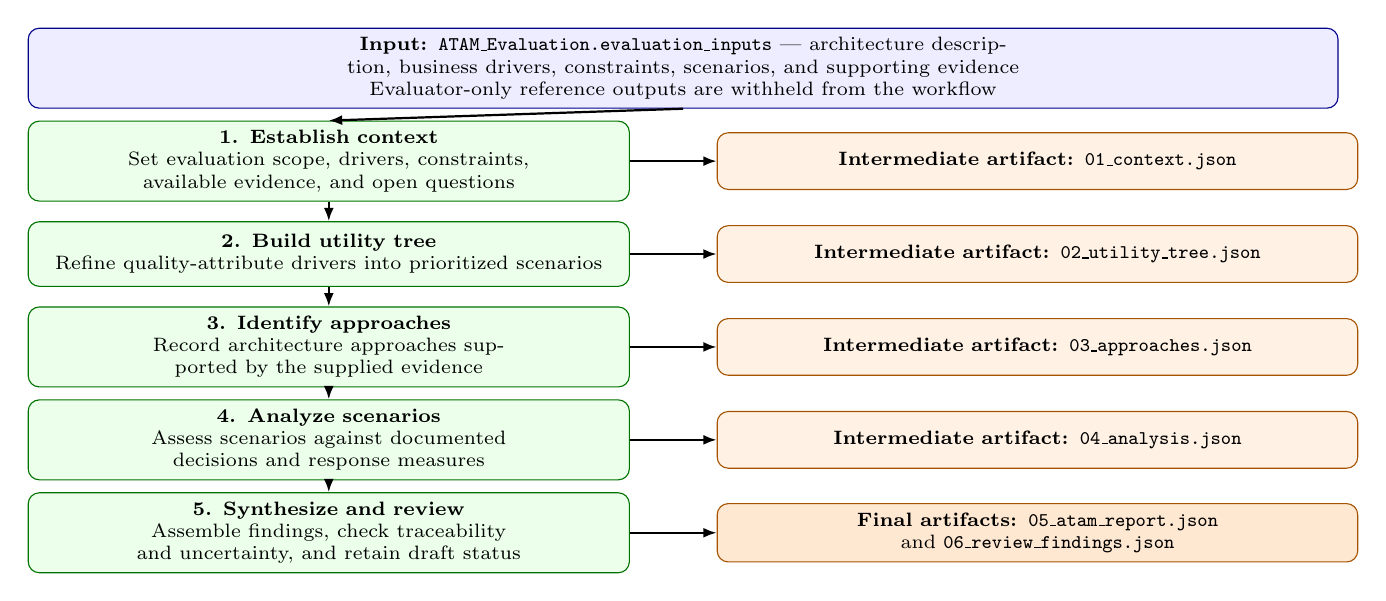
\begin{tikzpicture}[
  activity/.style={draw,rounded corners,align=center,text width=7.4cm,minimum height=0.82cm,font=\scriptsize,fill=green!8,draw=green!45!black},
  artifact/.style={draw,rounded corners,align=center,text width=7.9cm,minimum height=0.72cm,font=\scriptsize,fill=orange!10,draw=orange!65!black},
  caseinput/.style={draw,rounded corners,align=center,text width=16.4cm,minimum height=0.75cm,font=\scriptsize,fill=blue!7,draw=blue!55!black},
  arrow/.style={-{Latex[length=1.7mm]},thick}
]
\node[caseinput] (atamin) at (8.65,0) {\textbf{Input:} \texttt{ATAM\_Evaluation.evaluation\_inputs} --- architecture description, business drivers, constraints, scenarios, and supporting evidence\\Evaluator-only reference outputs are withheld from the workflow};
\node[activity] (atam1) at (4.15,-1.18) {\textbf{1. Establish context}\\Set evaluation scope, drivers, constraints, available evidence, and open questions};
\node[artifact] (atamout1) at (13.15,-1.18) {\textbf{Intermediate artifact:} \texttt{01\_context.json}};
\node[activity] (atam2) at (4.15,-2.36) {\textbf{2. Build utility tree}\\Refine quality-attribute drivers into prioritized scenarios};
\node[artifact] (atamout2) at (13.15,-2.36) {\textbf{Intermediate artifact:} \texttt{02\_utility\_tree.json}};
\node[activity] (atam3) at (4.15,-3.54) {\textbf{3. Identify approaches}\\Record architecture approaches supported by the supplied evidence};
\node[artifact] (atamout3) at (13.15,-3.54) {\textbf{Intermediate artifact:} \texttt{03\_approaches.json}};
\node[activity] (atam4) at (4.15,-4.72) {\textbf{4. Analyze scenarios}\\Assess scenarios against documented decisions and response measures};
\node[artifact] (atamout4) at (13.15,-4.72) {\textbf{Intermediate artifact:} \texttt{04\_analysis.json}};
\node[activity] (atam5) at (4.15,-5.90) {\textbf{5. Synthesize and review}\\Assemble findings, check traceability and uncertainty, and retain draft status};
\node[artifact,fill=orange!18] (atamout5) at (13.15,-5.90) {\textbf{Final artifacts:} \texttt{05\_atam\_report.json} and \texttt{06\_review\_findings.json}};
\draw[arrow] (atamin.south) -- (atam1.north);
\draw[arrow] (atam1.south) -- (atam2.north);
\draw[arrow] (atam2.south) -- (atam3.north);
\draw[arrow] (atam3.south) -- (atam4.north);
\draw[arrow] (atam4.south) -- (atam5.north);
\draw[arrow] (atam1.east) -- (atamout1.west);
\draw[arrow] (atam2.east) -- (atamout2.west);
\draw[arrow] (atam3.east) -- (atamout3.west);
\draw[arrow] (atam4.east) -- (atamout4.west);
\draw[arrow] (atam5.east) -- (atamout5.west);
\end{tikzpicture}%
}
\caption{ATAM evaluation workflow and artifact flow. Green boxes show method activities; blue shows runtime input; orange boxes name the artifacts written at each step. The figure summarizes the five method activities; the Claude Code realization separates synthesis, checking, and revision into additional runtime steps.}
\label{fig:atam-workflow}
\end{figure*}

\begin{figure*}[t]
\centering
\resizebox{\textwidth}{!}{%
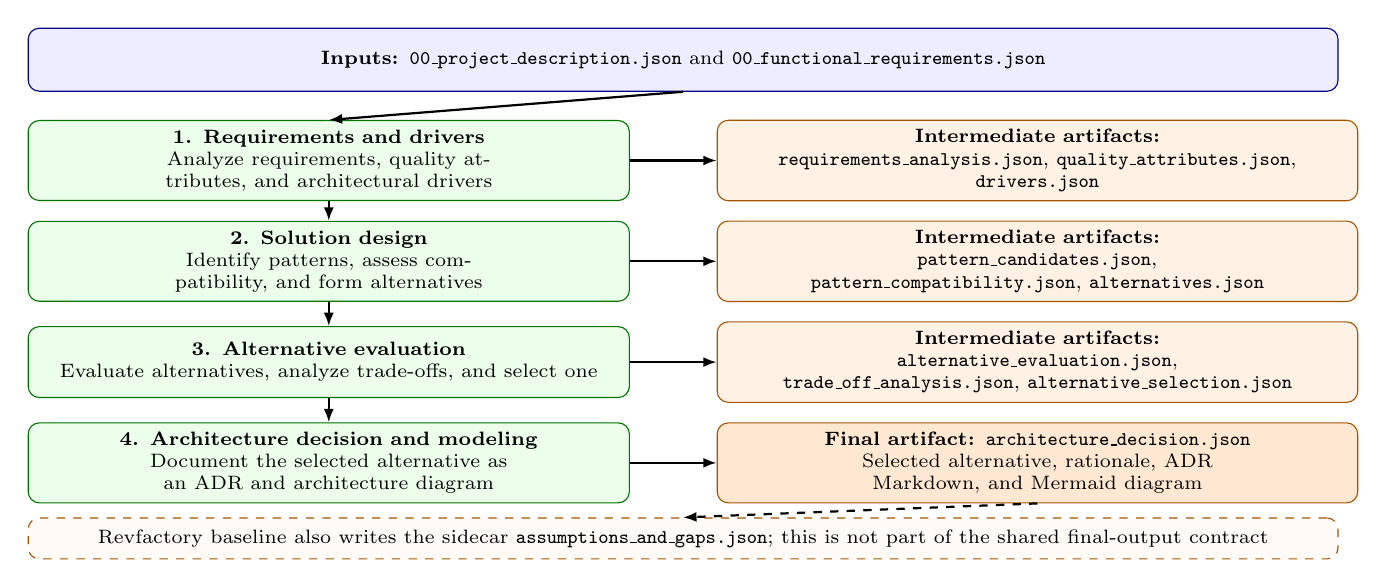
\begin{tikzpicture}[
  activity/.style={draw,rounded corners,align=center,text width=7.4cm,minimum height=0.9cm,font=\scriptsize,fill=green!8,draw=green!45!black},
  artifact/.style={draw,rounded corners,align=center,text width=7.9cm,minimum height=0.86cm,font=\scriptsize,fill=orange!10,draw=orange!65!black},
  caseinput/.style={draw,rounded corners,align=center,text width=16.4cm,minimum height=0.8cm,font=\scriptsize,fill=blue!7,draw=blue!55!black},
  sidecar/.style={draw,rounded corners,dashed,align=center,text width=16.4cm,minimum height=0.52cm,font=\scriptsize,fill=orange!4,draw=orange!65!black},
  arrow/.style={-{Latex[length=1.7mm]},thick}
]
\node[caseinput] (sarain) at (8.65,0) {\textbf{Inputs:} \texttt{00\_project\_description.json} and \texttt{00\_functional\_requirements.json}};
\node[activity] (sara1) at (4.15,-1.28) {\textbf{1. Requirements and drivers}\\Analyze requirements, quality attributes, and architectural drivers};
\node[artifact] (saraout1) at (13.15,-1.28) {\textbf{Intermediate artifacts:}\\\texttt{requirements\_analysis.json}, \texttt{quality\_attributes.json},\\\texttt{drivers.json}};
\node[activity] (sara2) at (4.15,-2.56) {\textbf{2. Solution design}\\Identify patterns, assess compatibility, and form alternatives};
\node[artifact] (saraout2) at (13.15,-2.56) {\textbf{Intermediate artifacts:}\\\texttt{pattern\_candidates.json},\\\texttt{pattern\_compatibility.json}, \texttt{alternatives.json}};
\node[activity] (sara3) at (4.15,-3.84) {\textbf{3. Alternative evaluation}\\Evaluate alternatives, analyze trade-offs, and select one};
\node[artifact] (saraout3) at (13.15,-3.84) {\textbf{Intermediate artifacts:}\\\texttt{alternative\_evaluation.json},\\\texttt{trade\_off\_analysis.json}, \texttt{alternative\_selection.json}};
\node[activity] (sara4) at (4.15,-5.12) {\textbf{4. Architecture decision and modeling}\\Document the selected alternative as an ADR and architecture diagram};
\node[artifact,fill=orange!18] (saraout4) at (13.15,-5.12) {\textbf{Final artifact:} \texttt{architecture\_decision.json}\\Selected alternative, rationale, ADR Markdown, and Mermaid diagram};
\node[sidecar] (sarasidecar) at (8.65,-6.08) {Revfactory baseline also writes the sidecar \texttt{assumptions\_and\_gaps.json}; this is not part of the shared final-output contract};
\draw[arrow] (sarain.south) -- (sara1.north);
\draw[arrow] (sara1.south) -- (sara2.north);
\draw[arrow] (sara2.south) -- (sara3.north);
\draw[arrow] (sara3.south) -- (sara4.north);
\draw[arrow] (sara1.east) -- (saraout1.west);
\draw[arrow] (sara2.east) -- (saraout2.west);
\draw[arrow] (sara3.east) -- (saraout3.west);
\draw[arrow] (sara4.east) -- (saraout4.west);
\draw[arrow,dashed] (saraout4.south) -- (sarasidecar.north);
\end{tikzpicture}%
}
\caption{SARA architecture-design workflow and artifact flow. Green boxes show the four method stages; blue shows the two case inputs; orange boxes show the intermediate and final artifacts. The dashed sidecar is an addition in the Revfactory baseline, not part of the shared final-output contract.}
\label{fig:sara-workflow}
\end{figure*}

\subsection{Execution evidence}

For HarnessWeaver's ATAM workflow, the recorded Claude Code and DeepAgents reports both passed the configured schema, ATAM-pilot, and reference-leakage checks after human corrections. The Claude corrections filled an empty \texttt{addressed\_attributes} field and replaced raw input paths in evidence citations with artifact IDs. The DeepAgents report received a post-run evidence correction and was synchronized with its stage artifact. Both outputs remain drafts awaiting architect review. These checks assess configured properties; they do not establish the substantive correctness of the analysis.

A separate Revfactory/harness baseline execution used Claude Code but did not use the HarnessWeaver-generated target bundle. Its schema and reference-leakage checks passed, while its ATAM check could not match 19 analysis records to source scenarios. This baseline observation is reported separately and is not evidence about HarnessWeaver's Claude materialization.

The SARA CampusBike case was generated from one saved HarnessSpec v0.2 for both targets. Each four-stage execution completed. The Claude Code output was \texttt{output/report.json}; the DeepAgents output was \texttt{output/architecture\_decision.json}. Both passed the available schema and reference-leakage checks. Both selected A3, but their rationales differ: the HarnessWeaver Claude result reports A1 and A3 each satisfy 10 of 13 requirements, while DeepAgents says A3 satisfies all stated requirements.

The same Revfactory Claude bundle was run twice. The first run resumed after a usage limit, used general-purpose agents for the remaining reviews, and packaged by a direct \texttt{jq} copy; it selected A3 and reported 12 of 13 requirements satisfied. Although the launcher record retains a failed exit status for the initial limit interruption, the resumed run log records completion and the final package review passed. The second run completed in one session with the configured stage and review agents, required no repairs, and passed schema and leakage checks; it selected A1 with 10 of 13 requirements satisfied. Both executions have recorded schema and leakage passes, and both final reviews recorded the same non-blocking concern that the diagram asserts HTTP/REST without input support. The different selections show that the generated baseline did not produce a stable decision across these two executions. Neither the SARA case nor its outputs have a domain-specific reference checker, and no result here is an independently validated architecture recommendation.

\begin{table*}[t]
\centering\footnotesize\renewcommand{\arraystretch}{1.12}
\begin{tabularx}{\textwidth}{>{\raggedright\arraybackslash}p{0.17\textwidth} >{\raggedright\arraybackslash}p{0.17\textwidth} >{\raggedright\arraybackslash}X >{\raggedright\arraybackslash}X}
\toprule
Case / target & Execution result & Available checks & Qualification\tabularnewline
\midrule
ATAM / Claude Code (HarnessWeaver) & Draft report produced & Schema, ATAM, leakage: pass after corrections & Architect review pending\tabularnewline
ATAM / DeepAgents (HarnessWeaver) & Five stages completed; draft report & Schema, ATAM, leakage: pass after correction & Architect review pending\tabularnewline
ATAM / Claude Code (Revfactory baseline) & Draft report produced & Schema and leakage: pass; 19 analysis records unmatched by ATAM check & Separate baseline run; not the HarnessWeaver target\tabularnewline
SARA / Claude Code & Four stages completed; A3 selected & Schema and leakage: pass & No domain checker or evaluator-only references; rationale differs from DeepAgents\tabularnewline
SARA / DeepAgents & Four stages completed; A3 selected & Schema and leakage: pass & No domain checker or evaluator-only references; rationale differs from Claude Code\tabularnewline
SARA / Revfactory Claude (run 1) & Resumed run; A3 selected (12/13) & Schema and leakage: pass; package review passed & Initial launcher status is failed (usage limit); general-purpose review agents and direct \texttt{jq} packaging on resume\tabularnewline
SARA / Revfactory Claude (run 2) & Four stages completed; A1 selected (10/13) & Schema and leakage: pass & One non-blocking unsupported protocol finding; no repairs\tabularnewline
\bottomrule
\end{tabularx}
\end{table*}

\textbf{Table II.} Recorded generation and execution evidence. Configured checks establish only the properties they encode; they do not establish expert acceptance, output quality, or behavioral equivalence.

\subsection{Preliminary interpretation}

The cases show that shared domain and methodology specifications can guide materialization and execution in both Claude Code and DeepAgents for two architecture workflows. The SARA HarnessWeaver targets selected the same alternative but gave different requirement-satisfaction rationales. The two executions of the same Revfactory baseline bundle selected different alternatives, A3 and A1, with different qualitative requirement counts. This observed variation cautions against treating a single generated report as a stable outcome. ATAM needed human corrections before all configured checks passed, and SARA has no domain-specific checker or evaluator-only reference set. These observations support feasibility as a prototyping approach, but do not demonstrate behavioral parity, improved quality, or reduced effort.

\section{Discussion and Research Agenda}

We treat the case as a \textbf{qualitative, artifact-centered feasibility evaluation}, supplemented by deterministic checks. It is not a controlled comparison and does not test hypotheses about productivity or output quality. Instead of presenting formal research questions that the current evidence cannot answer, we use three evaluation questions to organize what the case can show:

\begin{itemize}

\item
  \textbf{EQ1---Specification-to-runtime feasibility:} What parts of the ATAM and SARA intent, methodology, artifact contracts, and evidence rules can be materialized and executed in each target?
\item
  \textbf{EQ2---Reuse and target-specific work:} Which source assets remain shared, and what target-specific files, workflow adaptations, failures, or manual interventions appear across the two cases?
\item
  \textbf{EQ3---Method traceability and runtime differences:} How do generated workflows carry method activities and artifacts, and where do checks, explanations, or review behavior differ?
\end{itemize}

The current evidence gives descriptive answers only. The HarnessWeaver ATAM results passed the configured checks after human corrections, while the separately generated Revfactory baseline failed ATAM scenario matching. Both SARA runs completed and passed available schema checks, but their A3 recommendations differ in the rationale for requirement coverage. SARA has neither a domain-specific checker nor evaluator-only references. No measured results establish development or adaptation effort, assistant quality, expert agreement, or behavioral equivalence. Answering these questions requires repeated comparable tasks and explicit recording of models, prompts, runtimes, interventions, and artifacts. Future work should also exercise the \texttt{evolve} skill by applying execution or review feedback, regenerating workflows, and tracing which changes appear in later artifacts and checks.

\subsection{Threats to Validity}

\textbf{Construct validity.} Bundle checks and configured schema/domain checks provide evidence about structural conformance and selected ATAM rules. They do not directly measure methodological completeness, architect usefulness, or assistant quality. The ATAM results required human correction. SARA's schema and leakage checks do not evaluate domain correctness, and its case contains no evaluator-only reference outputs. These checks are therefore limited proxies for workflow quality.

\textbf{Internal validity.} The runtimes used different models and orchestration strategies, generation was interactive, and ATAM outputs received manual corrections. The first SARA baseline run was interrupted and resumed with general-purpose reviewers and manual packaging; the second used the configured agents. The two baseline outcomes differed, while the HarnessWeaver SARA outputs also differed in how they justified A3. These factors prevent attributing differences to the shared specification or runtime mapping alone. Two baseline runs are too few to characterize outcome variability.

\textbf{External validity.} The evaluation covers two architecture methods, one case for each method, and two runtime technologies. The observations may not generalize to other domains, inputs, models, or runtime environments.

\textbf{Reliability.} LLM outputs and interactive generation can vary across runs and software versions. We preserve source and bundle records, prompts, check results, and manual interventions, but have not established repeatability across independent generations or executions.

Further evaluation should add domain-specific checks and reference outputs for SARA, compare review and revision behavior across targets, exercise the \texttt{evolve} skill, measure design and implementation effort, record manual interventions, and repeat runs to assess variability. The current work does not claim automatic optimal workflow discovery, broad design-space exploration, or generator learning.

\section{Conclusion}

HarnessWeaver is an exploratory model-based approach for describing domain-specific agentic workflows and materializing them as LLM-based assistants in different runtimes. The ATAM and SARA cases demonstrate workflow prototypes in Claude Code and DeepAgents from shared specifications. For SARA, both HarnessWeaver targets selected A3, while two executions of the Revfactory Claude baseline selected A3 and A1, respectively. This provides an initial observation of decision variability and shows why output review and repeated runs matter. The ATAM targets passed configured checks after corrections; the SARA runs passed their available schema and leakage checks, which do not assess domain correctness. The evidence does not measure effort or establish output quality or behavioral equivalence, and the reports have not received independent architect sign-off. Future work should evaluate the \texttt{evolve} skill, add stronger domain validation, measure effort and repeatability, and examine whether these generated workflows should be classified as agent harnesses and what properties would justify that classification.

\balance
\bibliographystyle{IEEEtran}
\bibliography{references}
\end{document}
